\section{Methods}
\label{sec:methods}

% Overview
CLAM and CHAODA comprise many components, all described in this section.
We start with a brief overview of those components.
CLAM begins with a dataset and a distance metric, to which it applies hierarchical clustering to build a tree.
CLAM selects clusters from the tree using meta-machine-learning (meta-ml) models trained\footnote{Note that during training, CHAODA is somewhat supervised.
CHAODA uses this training to learn a set of meta-ml models for selecting clusters and inducing graphs.
During testing, and inference, on new datasets, CHAODA is unsupervised and uses the learned meta-ml models.} according to several geometric and topological properties.
These meta-ml models learn relationships between these properties and expected anomaly-detection performance.
CLAM then induces graphs from the selected clusters.
CHAODA applies its constituent algorithms to these graphs, and combines the individual scores into an ensemble, ultimately producing anomaly scores for each datum.
See Figure~\ref{fig:methods:chaoda-workflow} for a high-level illustration.


\begin{figure*}[ht!]
    \centering
    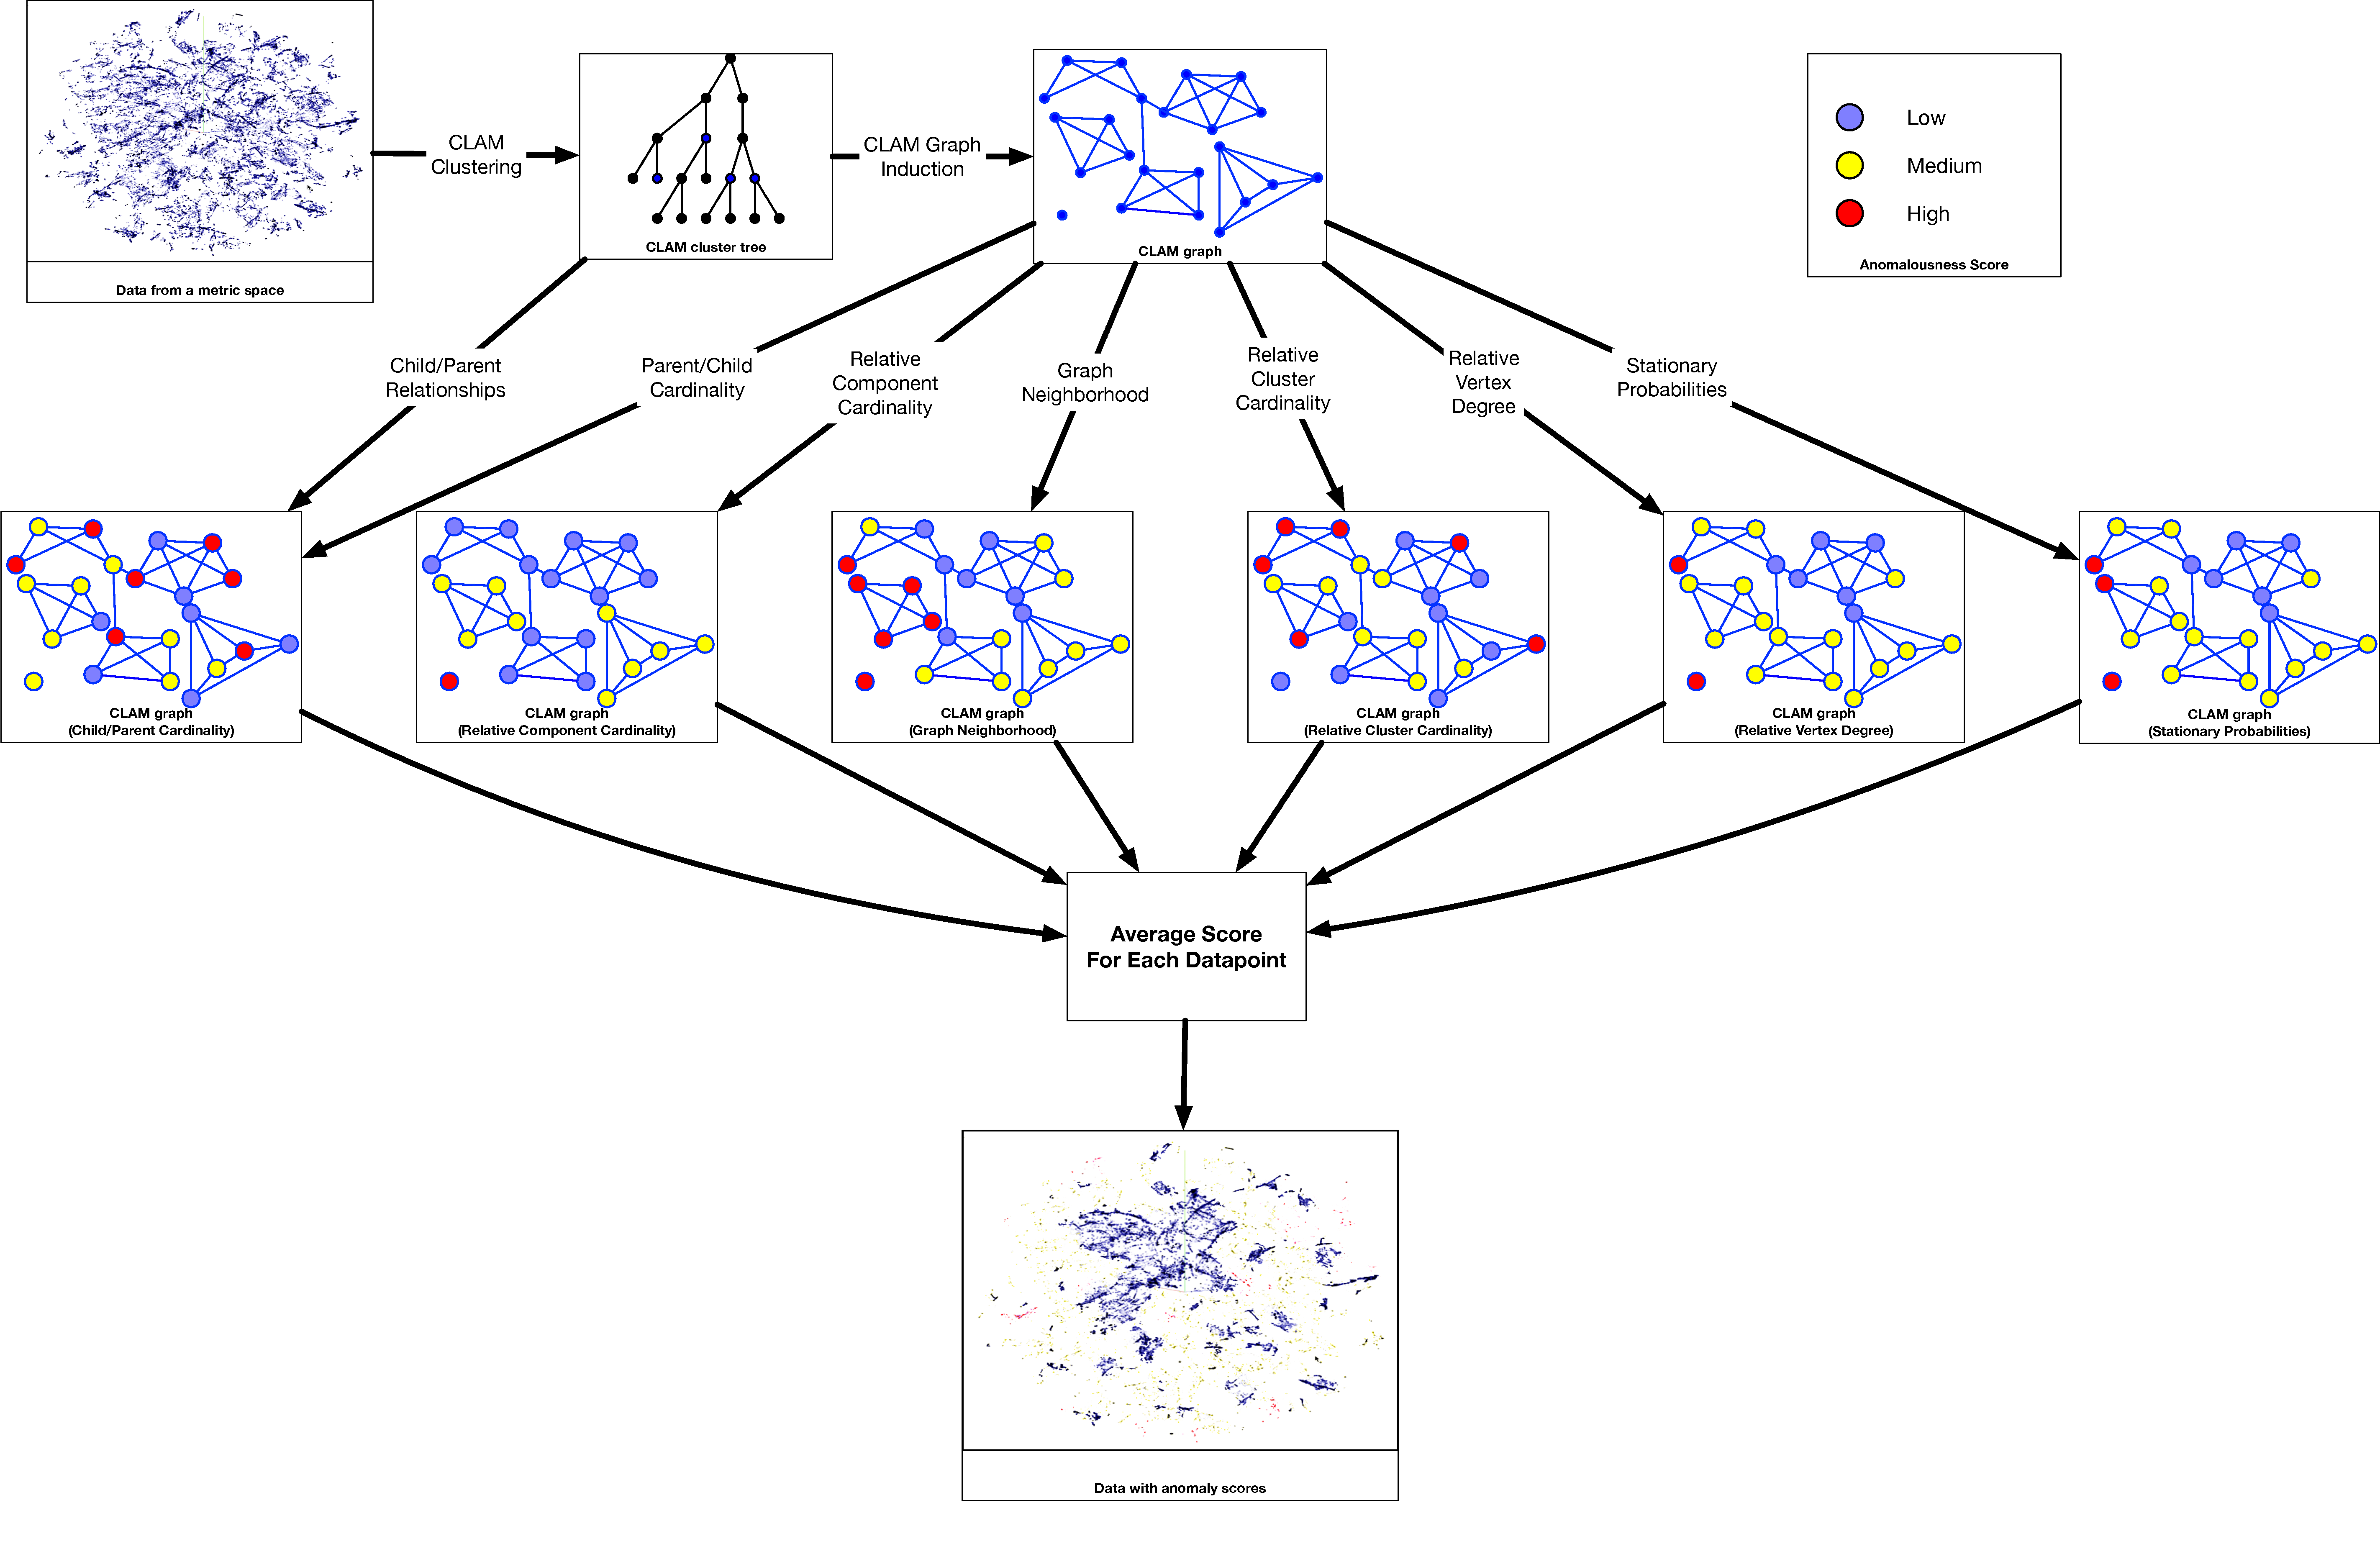
\includegraphics[width=6in]{images/chaoda-workflow.pdf}
    \caption{\textbf{Overview of the CHAODA workflow.}
        Beginning with a dataset and a distance metric, CLAM builds a cluster tree and induces several graphs from this tree; for the sake of simplicity, we illustrate only one such graph here.
        Each of CHAODA's constituent algorithms provides distinct anomaly scores on its graph.
        These scores are normalized and aggregated into a final score for each cluster, and by extension, each datum.
        In this figure, we have simplified the scores to a ternary color scheme; actual scores are real-valued between 0 and 1.
        Note that each algorithm provides its own scoring, but there may be similarities such as between vertex degree and stationary distribution.}
    \label{fig:methods:chaoda-workflow}
\end{figure*}

\subsection{Dataset and Distance Function}
\label{subsec:methods:dataset-and-distance-function}

We start with a dataset $\textbf{X} = \{x_1 \dots x_n\}$ with $n$ points and a distance function $f : (\textbf{X}, \textbf{X}) \mapsto \mathbb{R}^+$.
The distance function takes two points from the dataset and deterministically produces a non-negative real number.
We also require the distance function to be symmetric and for the distance between two identical points to be zero, i.e., $\forall x, y \in X$, $f(x, y) = f(y, x)$ and $f(x, y) = 0 \Leftrightarrow x = y$.
CLAM and CHAODA are general over any distance function that obeys these constraints.

CLAM assumes the ``manifold hypothesis''~\cite{fefferman2016testing}, i.e.\ datasets collected from constrained generating phenomena that are embedded in a high-dimensional space typically only occupy a low-dimensional manifold in that space.
CLAM and CHAODA learn the geometric and topological properties of these manifolds in a way that generalizes across datasets and distance function regardless of dataset-specific properties such as total number of points, dimensionality, absolute distance values, etc.
We demonstrate this genericity by our anomaly detection performance in Section~\ref{sec:results}.

Note that we often speak of each datum as embedded in a $D$-dimensional metric space and we use Euclidean notions, such as voids and volumes, to talk about the geometric and topological properties of the manifold.
The purpose of such notions is to help build intuition and to aid understanding.
Mathematically, CLAM does not rely on such notions; in-fact, the details of an embedding space can be abstracted away behind the distance function.

Also note that we can provide certain guarantees (see CHESS~\cite{ishaq2019clustered}) when the distance function is a metric, i.e.\ it obeys the triangle inequality.
While CLAM and CHAODA work well with distance functions that are not metrics, we have not investigated how the lack of the triangle inequality changes, or breaks, those guarantees in the context of anomaly detection.
For this paper, we show results using the $L1$-norm and $L2$-norm.


\subsection{Clustering}
\label{subsec:methods:clustering}

We start by building a divisive hierarchical clustering of the dataset.
We partition, as described in Algorithm~\ref{alg:partition}, a cluster with $k$ points using a pair of well-separated points from among a random sampling of $\sqrt k$ points.
Starting from a root-cluster containing the entire dataset, we continue until each leaf contains only one datum.
This achieves clustering in expected $\mathcal{O}(n \lg n)$ time.
This procedure improves upon the clustering approach from CHESS~\cite{ishaq2019clustered} by a better selection of maximally-separated points, and by memoizing critical information about each cluster (discussed below).

\begin{algorithm} % enter the algorithm environment
\caption{Partition} % give the algorithm a caption
\label{alg:partition} % and a label for \ref{} commands later in the document
\begin{algorithmic}[1] % enter the algorithmic environment
    \REQUIRE $cluster$
    \STATE $k \leftarrow \lfloor \sqrt{|cluster.points|} \rfloor$
    \STATE $seeds \leftarrow k$ random points from $cluster.points$
    \STATE $c \leftarrow$ geometric median of $seeds$
    \STATE $r \leftarrow \argmax d(c,x) \ \forall \ x \in cluster.points$
    \STATE $l \leftarrow \argmax d(r,x) \ \forall \ x \in cluster.points$
    \STATE $left \leftarrow \{x | x \in cluster.points \land d(l,x) \le d(r,x)\}$
    \STATE $right \leftarrow \{x | x \in cluster.points \land d(r,x) < d(l,x)\}$
    \IF{$|left| > 1$}
        \STATE Partition($left$)
    \ENDIF
    \IF{$|right| > 1$}
        \STATE Partition($right$)
    \ENDIF
\end{algorithmic}
\end{algorithm}

These clusters have several interesting and important properties for us to consider.
These include the \textit{cardinality}, the number of points in a cluster;
\textit{center}, the approximate geometric median of points contained in a cluster;
\textit{radius}, the distance to the farthest point from the center;
and \textit{local fractal dimension},
as given by:

\begin{gather}
    \log_2\bigg(\frac{|B_X(c, r)|}{|B_X(c, \frac{r}{2})|}\bigg)
    \label{fractal-dimension}
\end{gather}

where $B_X(c,r)$ is the set of points contained in a ball of radius $r$ on the dataset $X$ centered on a point $c$~\cite{ishaq2019clustered}.
Thus, local fractal dimension captures the ``spread'' of points on the manifold in comparison to the (typically much larger) embedding space.
This is motivated by the idea that the induced graphs will learn to adapt to use different ``resolutions'' to characterize different regions of the manifold (see Figure~\ref{fig:methods:cluster-resolution}).

We can also consider \textit{child-parent ratios} of the cardinality, radius, and local fractal dimension of a cluster, as well as the \textit{exponential moving averages} of those child-parent ratios along a branch of the tree.
In particular, we use the child-parent ratios and their exponential moving averages to help CHAODA generalize from a small set of training datasets to a large, distinct set of testing datasets.
During clustering, we memoize these ratios as we create each cluster.
CHAODA can then make direct use of these ratios to aid in anomaly detection.


\subsection{Graphs}
\label{subsec:methods:graphs}

Clusters that are close together sometimes have overlapping volumes; i.e.,\ the distance between their centers is less than or equal to the sum of their radii.
We define a graph $G=(V,E)$ with vertices in one-to-one correspondence to CLAM clusters and with an edge between two vertices if and only if their corresponding clusters overlap.
While it is fairly standard in the literature to define graphs in this way, the challenge lies in selecting the right clusters to build useful graphs.
Our selection process, presented in Section~\ref{subsec:methods:cluster-selection-for-graphs}, is among the major novel contributions of CLAM and CHAODA.

In the context of graphs, we use the terms \textit{cluster} and \textit{vertex} interchangeably.
By \textit{graph cardinality} we mean \textit{vertex cardinality}, i.e., the number of clusters in the graph, and by \textit{graph population} we mean the sum of cardinalities of all clusters in the graph.
Note that \textit{cluster cardinality} refers to the number of points within a cluster.
We use \textit{layer-graph} to refer to a graph built from clusters at a fixed depth from the tree and \textit{optimal-graph} to refer to a graph built from clusters selected by the processes described in Section~\ref{subsec:methods:cluster-selection-for-graphs}.

Figure~\ref{fig:methods:graph-generation} illustrates how CLAM induces a graph from non-uniform depths in a cluster tree, while Figure~\ref{fig:methods:cluster-resolution} illustrates how, if clusters are chosen at the right ``resolution,'' these graphs can capture the structure of the manifold.
Interestingly, the clusters are not necessarily hyperspheres, but polytopes akin to a high-dimensional Voronoi diagram~\cite{voronoi1908nouvelles}.
The induced graph need not be fully connected and, in practice, often contains many small, disjoint connected components.

\begin{figure}[ht!]
    \centering
    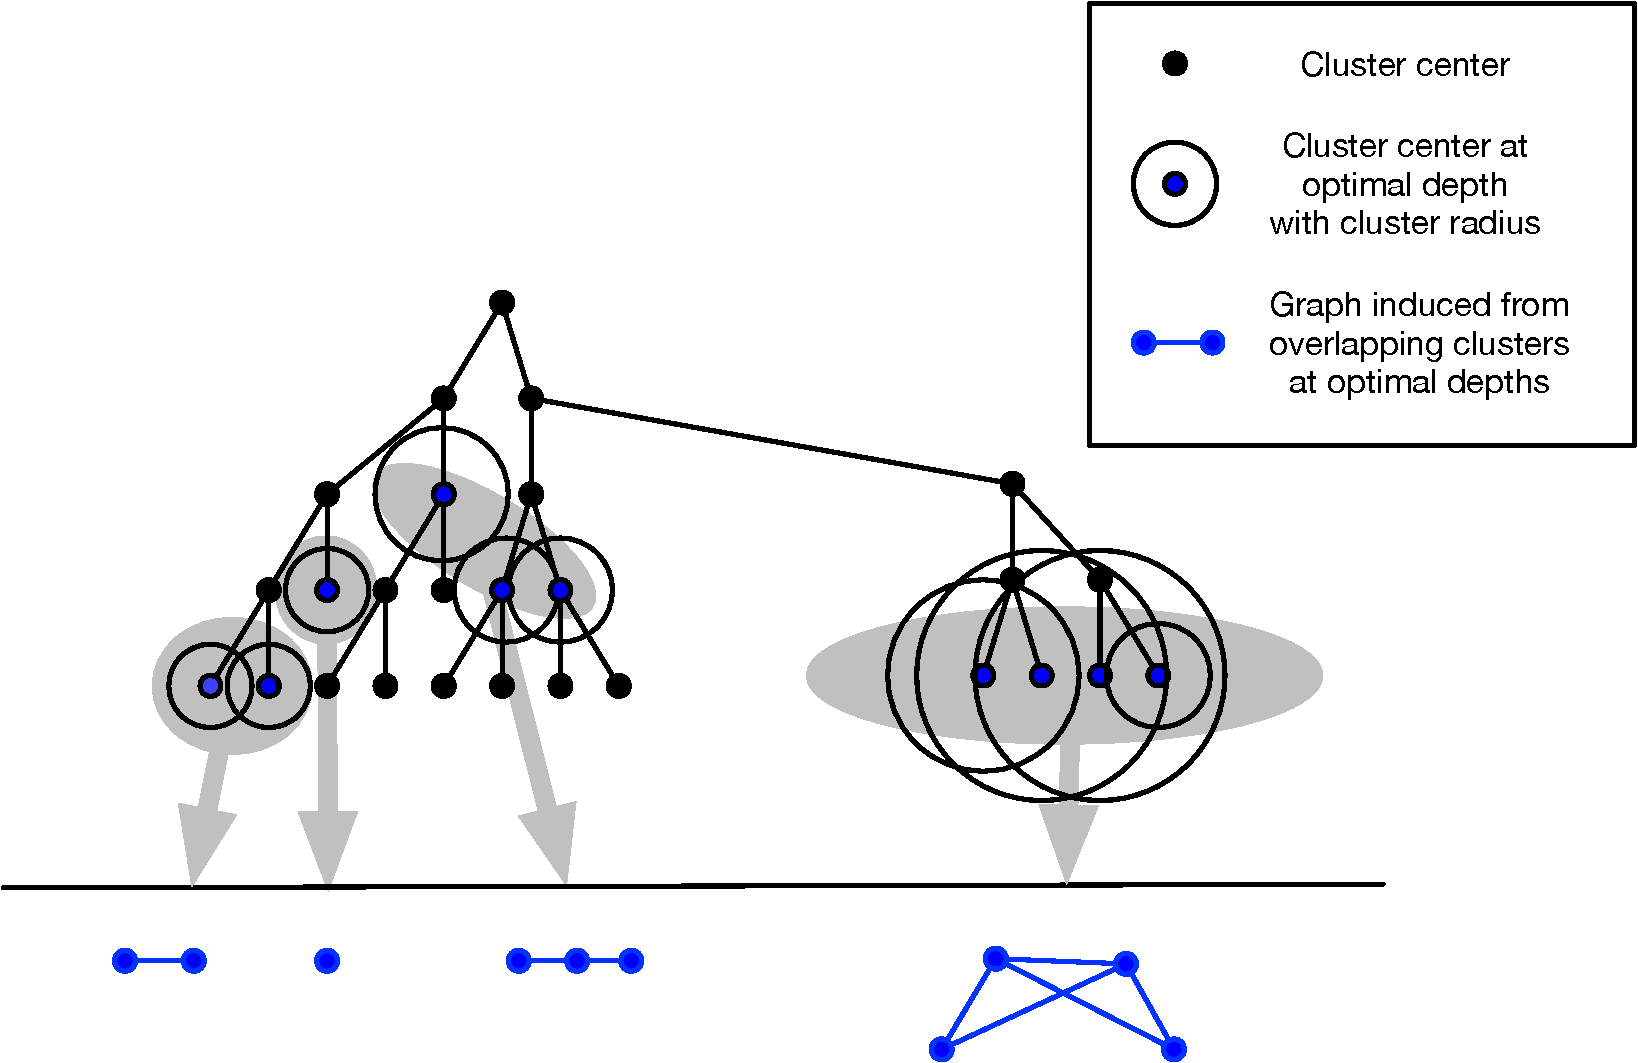
\includegraphics[width=2.5in]{images/tree-graph.pdf}
    \caption{Using CLAM to induce a graph from a cluster tree.
        Dots in the tree represent cluster centers;
        blue dots represent centers of chosen clusters.
        Circles represent the volume of a cluster (the radius is the distance from the center to the furthest point contained within that cluster).
        Gray arrows point to the induced graph components, which are indicated in blue below the horizontal line.}
    \label{fig:methods:graph-generation}
\end{figure}

For our purposes, a CLAM graph exhibits an important invariant.
The clusters corresponding to vertices in the graph collectively contain every point in the dataset, and each point in the dataset is assigned to exactly one cluster in the graph.
A corollary to this invariant is that a graph will never contain two clusters such that one cluster is an ancestor or descendant of another cluster.
This also assures that a \textit{graph's population} is equal to the cardinality of the dataset, i.e. $|\textbf{X}|$ or $n$.

\begin{figure}[ht!]
    \centering
    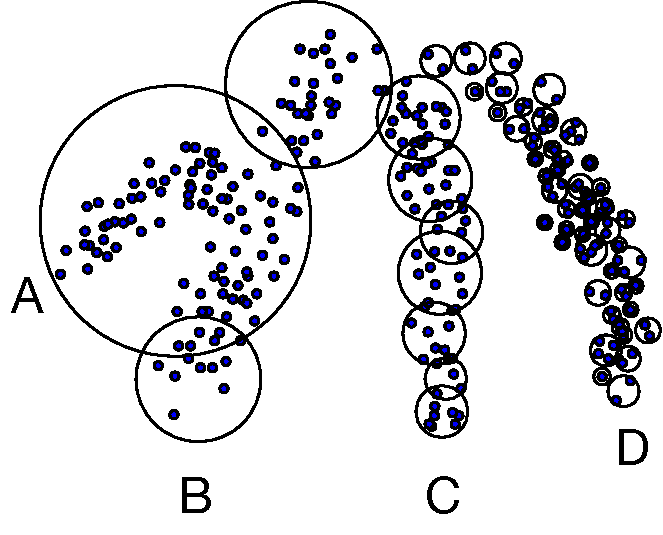
\includegraphics[width=2.5in]{images/cluster-resolution.pdf}\\
    \vspace{1cm}
    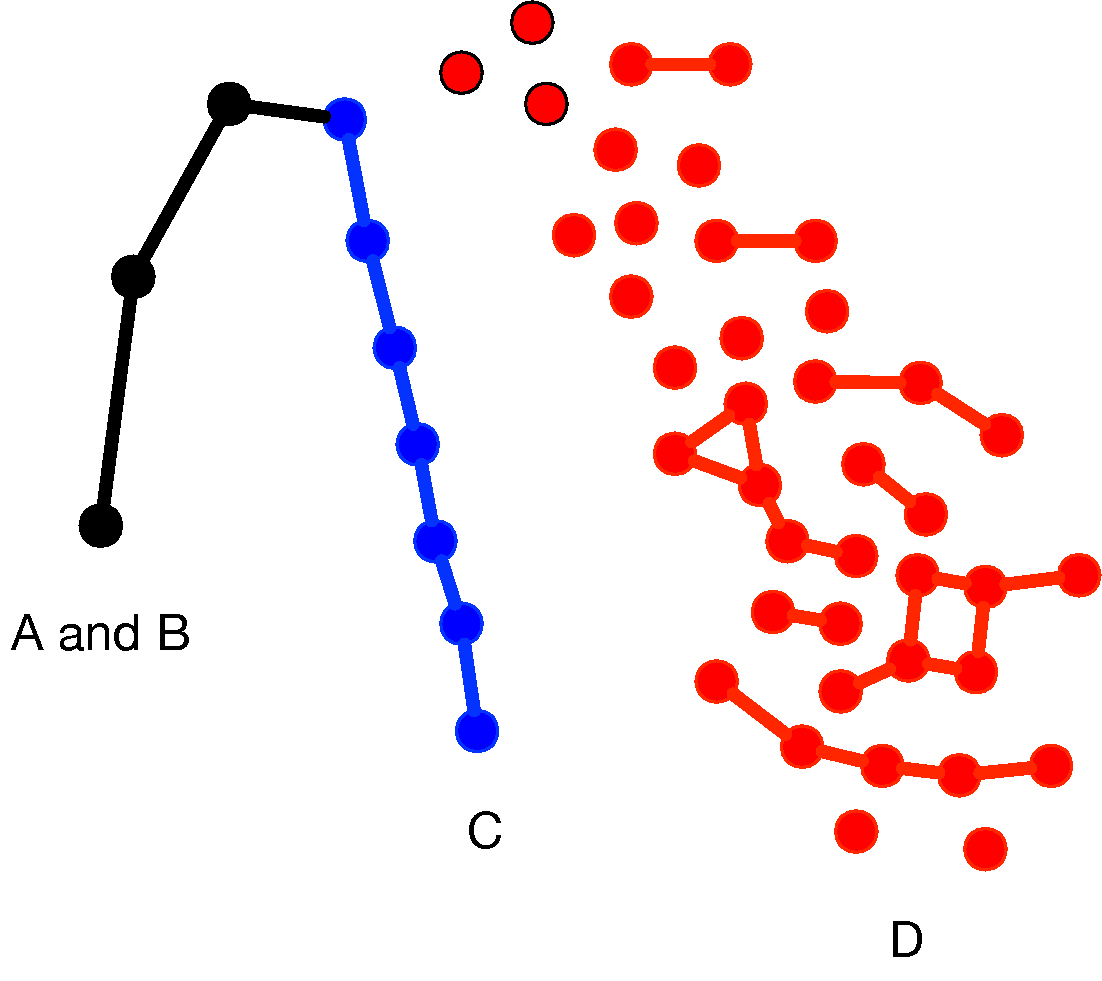
\includegraphics[width=2.5in]{images/cluster-resolution-graph.pdf}
    \caption{
        \textbf{Cluster resolution.}
        Consider this toy dataset whose manifold comprises the four named branches.
        In the top part of the figure, with each branch, we show clusters that we might get from different depths in the tree.
        Clusters on branches A and B come from low depths in the tree and have large voids, i.e.\ regions with no points in them.
        Clusters on branch D come from a high depth in the tree and are, in a sense, too small for the ``thickness'' of the branch they cover.
        Clusters on branch C are ``just right'' because their diameters are roughly equal to the thickness of the branch, and they contain no large voids.
        We can track how the local fractal dimension of these clusters changes as we traverse the tree and as we move along clusters that are adjacent on the manifold.
        In this way, changes in the local fractal dimension can serve as a proxy for deciding which clusters would help ``well characterize'' the underlying manifold.
        In the bottom part of the figure, we show the graphs CLAM would induce from these different clusters.
        Note that branches A and B are not distinguished; the separation between the branches is lost in the graph representation.
        A graph induced from branch D would consist of many disconnected subgraphs, and would not represent the structure of the entire branch.
        Finally, a graph induced from branch C represents the branch structure, including its connection to branches A and B.
    }
    \label{fig:methods:cluster-resolution}
\end{figure}


\subsection{Individual Algorithms}
\label{subsec:methods:individual-algorithms}

Given an induced graph that characterizes a manifold, we must extract information about the anomalousness of clusters in that graph.
Here we describe six simple algorithms for anomaly detection, each using a CLAM graph to calculate an anomalousness score for each cluster and datum.
Given that the key to an effective ensemble is for each member to contribute a unique inductive bias~\cite{chen2017outlier}, we also note the intuition behind each algorithm's contributions.
These scores can be used, along with the ground-truth labels, to compute the area under the curve (AUC) of the receiver operating characteristic (ROC)~\cite{fawcett2006introduction} to measure the anomaly detection performance of the graph which produced those scores.

In the following,
$V$ and $E$ are the sets of clusters and edges respectively in a graph,
$|c|$ is the cardinality of a cluster $c$,
and $|C|$ is the cardinality of a component $C$.
Each algorithm assigns an anomalousness score to each cluster.
Each point is then assigned the anomalousness score of the cluster it belongs to.
These scores are internally consistent for each individual algorithm, i.e.\ low scores indicate inliers and high scores indicate outliers.
However, different algorithms assign scores in wide, and often different, ranges of values.
We use Gaussian normalization to constrain the raw scores to a $[0, 1]$ range.
This lets us combine scores into an ensemble (see Section~\ref{subsec:methods:the-ensemble}).
See~\cite{kriegel2011interpreting} for a thorough discussion of anomaly-score normalization in ensemble methods.

The overall computational complexity of these algorithms appears in Table~\ref{table:methods:complexity}.

\begin{table}[ht!]
\centering
\caption{Time complexity of CHAODA algorithms.}
\label{table:methods:complexity}
\begin{tabular}{|l|l|}
\hline
\textbf{Algorithm} & \textbf{Complexity} \\
\hline
 Relative Cluster Cardinality & $\mathcal{O}(|V|)$ \\
 \hline
 Relative Component Cardinality & $\mathcal{O}(|E| + |V|)$  \\
 \hline
 Graph Neighborhood Size & $\mathcal{O}(|E| \cdot |V|)$  \\ 
 \hline
 Child-Parent Cardinality Ratio & $\mathcal{O}(|V|)$ \\ 
 \hline
 Stationary Probabilities & $\mathcal{O}(|V|^{2.37})$ \\ 
 \hline
 Relative Vertex Degree & $\mathcal{O}(|V|)$ \\
 \hline
\end{tabular}
\end{table}


\subsubsection{Relative Cluster Cardinality}
\label{subsubsec:methods:individual-algorithms:relative-cluster-cardinality}
We measure the anomalousness of a point by the cardinality of the cluster that the point belongs to relative to the cardinalities of the other clusters in the graph.
Points in the same cluster are considered equally anomalous.
Points in clusters with lower cardinalities are considered more anomalous than points in clusters with higher cardinalities.
Formally, $\forall c \in G, \ \score(c) = -|c|$.

The intuition is that points in clusters with higher cardinalities are close to each other, and thus are less likely to be anomalous.
The time complexity is $\mathcal{O}(|V|)$ because this requires a single pass over the clusters in a graph.


\subsubsection{Relative Component Cardinality}
\label{subsubsec:methods:individual-algorithms:relative-component-cardinality}
We use the usual definition of connected components:
no two vertices from different components have an edge between them and every pair of vertices in the same component has a path connecting them.
We consider points in clusters in smaller components to be more anomalous than points in clusters in larger components.
Points in clusters in the same component are considered equally anomalous.
Formally, $\forall C \in G, \ \forall c \in C,  \\score(c) = -|C|$.

The intuition here, as distinct from the previous algorithm, is to capture larger-scale structural information based on disjoint connected components from the graph.
The time complexity is $\mathcal{O}(|E| + |V|)$ because we first need to find the components of the graph using a single pass over the edges, and then score each cluster in the graph using a single pass over those clusters.


\subsubsection{Graph Neighborhood Size}
\label{subsubsec:methods:individual-algorithms:graph-neighborhood-size}
Given the graph, we consider the number of clusters reachable from a starting cluster within a given graph distance $k$, i.e.\ within $k$ hops along edges.
We call this number the \textit{graph-neighborhood size} of the starting cluster.
With $k$ small compared to the diameter of a component, we consider the relative graph-neighborhood-sizes of all clusters.
Clusters with small graph-neighborhoods are considered more anomalous than clusters with large graph-neighborhoods.

The intuition here is to capture information about the connectivity of the graph in the region around each cluster.
The computation is defined in Algorithm~\ref{alg:graph-neighborhood-size}.
Its time complexity is $\mathcal{O}(|E| \cdot |V|)$ because we need to compute the eccentricity of each cluster.

\begin{algorithm}[h]
    \caption{Graph Neighborhood}
    \label{alg:graph-neighborhood-size}
\begin{algorithmic}[1]
    \REQUIRE $G$, a graph
    \REQUIRE $\alpha \in \mathbb{R}$ in the range $(0,1]$ ($0.25$ by default).
    \FOR {cluster $c \in G$}
        \STATE $e_c \gets$ the eccentricity of $c$
        \STATE $s \gets e_c \cdot \alpha$  % Add \ceil operator
        \STATE perform a breadth-first traversal from $c$ with $s$ steps
        \STATE $v \gets$ the number of unique clusters visited
        \STATE $\score(c) \gets -v$
    \ENDFOR
\end{algorithmic}
\end{algorithm}


\subsubsection{Child-Parent Cardinality Ratio}
\label{subsubsec:methods:individual-algorithms:child-parent-cardinality-ratio}
As described in Section~\ref{subsec:methods:clustering}, the partition algorithm used in clustering splits a cluster into two children.
If a child cluster contains only a small fraction of its parent's points, then we consider that child cluster to be more anomalous.
These child-parent cardinality ratios are accumulated along each branch in the tree, terminating when the child cluster is among those selected in the graph.
Clusters with a low value of these accumulated ratios are considered more anomalous than clusters with a higher value.
Formally, $\forall c \in G, \ \score(c) = \frac{|p|}{|c|} + score(p)$ where $p$ is the parent cluster of $c$.

This algorithm was inspired by iForest~\cite{tony2008iforest}, and captures information from the tree and the graph.
Unlike the other individual algorithms, this accumulates parent scores into the children.
The time complexity of this algorithm is $\mathcal{O}(|V|)$, because these ratios are memoized during the clustering process and we need only look them up once for each cluster in the graph.


\subsubsection{Stationary Probabilities}
\label{subsubsec:methods:individual-algorithms:stationary-probabilities}
For each edge in the graph, we assign a weight inversely proportional to the distance between the centers of the two clusters that connect to form that edge.
The outgoing probabilities from a cluster are stochastic over the edge weights for that cluster.
We compute the transition probability matrix of each component that contains at least two clusters.
The process of successively squaring this matrix will converge~\cite{levin2017markov}.
We follow this process for each component in the graph and find the convergent matrix.
Consider the sum of the values along a row in this matrix.
This is the expected proportion of visits to that cluster during an infinitely long random walk over the component.
We consider this sum to be inversely related to the anomalousness of the corresponding cluster.

The intuition here is that clusters that are more difficult to reach during an infinite random walk are more likely to contain anomalous points.
The algorithm is defined in Algorithm~\ref{alg:stationary-probabilities}.
Its worst-case time complexity is $\mathcal{O}(|V|^{2.37})$ given by the matrix multiplication algorithm from~\cite{alman2021refined}.
In practice, however, this algorithm has much better performance than indicated by the theoretical complexity, because the induced graphs are often composed of several small components rather than one, or a few large, component(s).

\begin{algorithm}[h]
    \caption{Stationary Probabilities}
    \label{alg:stationary-probabilities}
\begin{algorithmic}[1]
    \REQUIRE $G$, a graph
    \FOR {component $C \in G$}
        \STATE $M \gets$ the transition matrix for $C$
        \REPEAT
            \STATE $M \gets M^2$
        \UNTIL $M$ converges
        \FOR {cluster $c \in C$}
            \STATE $s \gets $ the row from $M$ corresponding to $c$
            \STATE $\score(c) \gets -\Sigma(s)$ 
        \ENDFOR
    \ENDFOR
\end{algorithmic}
\end{algorithm}


\subsubsection{Relative Vertex Degree}
\label{subsubsec:methods:individual-algorithms:relative-vertex-degree}
For each cluster in the induced graph, consider its degree, i.e. the number of edges connecting to that cluster.
We consider a cluster with high degree to be less anomalous than a cluster with low degree.
This is essentially a version of the previous algorithm that ignores edge weights, and will have different biases with regard to the sampling density of the dataset.
Formally, $\forall c \in G, \ \score(c) = -\deg(c)$.
Its time complexity is $\mathcal{O}(|V|)$.


\subsection{Training Meta-Machine-Learning Models}
\label{subsec:methods:training-meta-ml-models}

Section~\ref{subsec:methods:clustering} makes note of some important geometric and topological properties of CLAM clusters, i.e.\ cardinality, radius and local fractal dimension.
We find the child-parent ratios of these properties and the exponential moving averages of these ratios along each branch in the tree.
Each child-parent ratio is obtained by dividing the value for the child by the value for the parent, e.g.\ $R= \frac{|child|}{|parent|}$.
Each new exponential moving average (EMA) is the weighted sum of the previous EMA and the current ratio.
Specifically, $ema_{i+1} = \alpha * R_{i + 1} + (1 - \alpha) * ema_i$ for some $\alpha \in [0, 1]$.
We chose an $\alpha$ of $\frac{2}{11}$.

Using these ratios instead of the raw values themselves makes CHAODA agnostic to dataset-specific properties; it need only consider how those properties change as we traverse the tree or a graph.
For a given graph, we can take the average values of the six ratios from its constituent clusters to form a feature-vector.
We can use the methods described in Section~\ref{subsec:methods:individual-algorithms} to compute the area under the ROC curve from using each individual algorithm to predict anomalousness scores from that graph.
Each pairing of the feature-vector and an ROC score forms a training sample for our meta-ml models.
We use linear regression and decision-tree regressors to fill the role of those meta-ml models.
We use these data to train the meta-ml models to predict the ROC score for a graph from its feature-vector.

We randomly selected six datasets whose cardinalities are between $10^3$ and $10^5$ for training, and we used the $L1$-norm and $L2$-norm for each dataset.
For each pairing of dataset and distance function, CLAM builds a new cluster-tree.
Meta-ml training then proceeds over several epochs, the first of which we seed with some layer graphs from each tree.
During each epoch, we extract the feature vector from each graph, and we find the ROC AUC of applying each individual algorithm to each graph.
Each pairing of feature-vector and ROC score forms a training sample.
For each pairing of dataset and distance function, we initialize a linear regressor and a decision-tree regressor to form our suite of meta-ml models.
We train each meta-ml model with every training sample collected thus far, for ten epochs.
We use the trained meta-ml models to select clusters (see Section~\ref{subsec:methods:cluster-selection-for-graphs}) for new graphs that are used for the next epoch.
We note that this was not $k$-fold cross validation, but a one-time selection of six datasets for training based on size as a selection criterion.

During the earlier epochs, we expect to have selected graphs that exhibit poor anomaly detection performance.
For later epochs, we expect this performance to improve.
With each epoch, we add to the set of training samples collected thus far and we train a new suite of meta-ml models for selecting better clusters.
This is so that the meta-ml models can learn to distinguish between ratios that select for low ROC AUC from those ratios that select for high ROC AUC.
Each meta-ml model sees training data from each pairing of dataset and distance function.
This lets CHAODA generalize across different datasets and distance functions.


\subsection{Cluster Selection for Graphs}
\label{subsec:methods:cluster-selection-for-graphs}

The heart of the problem with CHAODA is in selecting the ``right'' clusters that would build a graph that provides a useful representation of the underlying manifold.
One could try every possible combination of clusters to build graphs, but this quickly leads to combinatorial explosion.
Instead, CHAODA focuses on intelligently selecting clusters for a graph which is expected to perform well for anomaly detection.
Area under the curve (AUC) of the receiver operating characteristic (ROC) is often used to benchmark anomaly detectors~\cite{fawcett2006introduction}.
CHAODA selects clusters to optimize for this measure.

\begin{figure}[ht!]
    \centering
    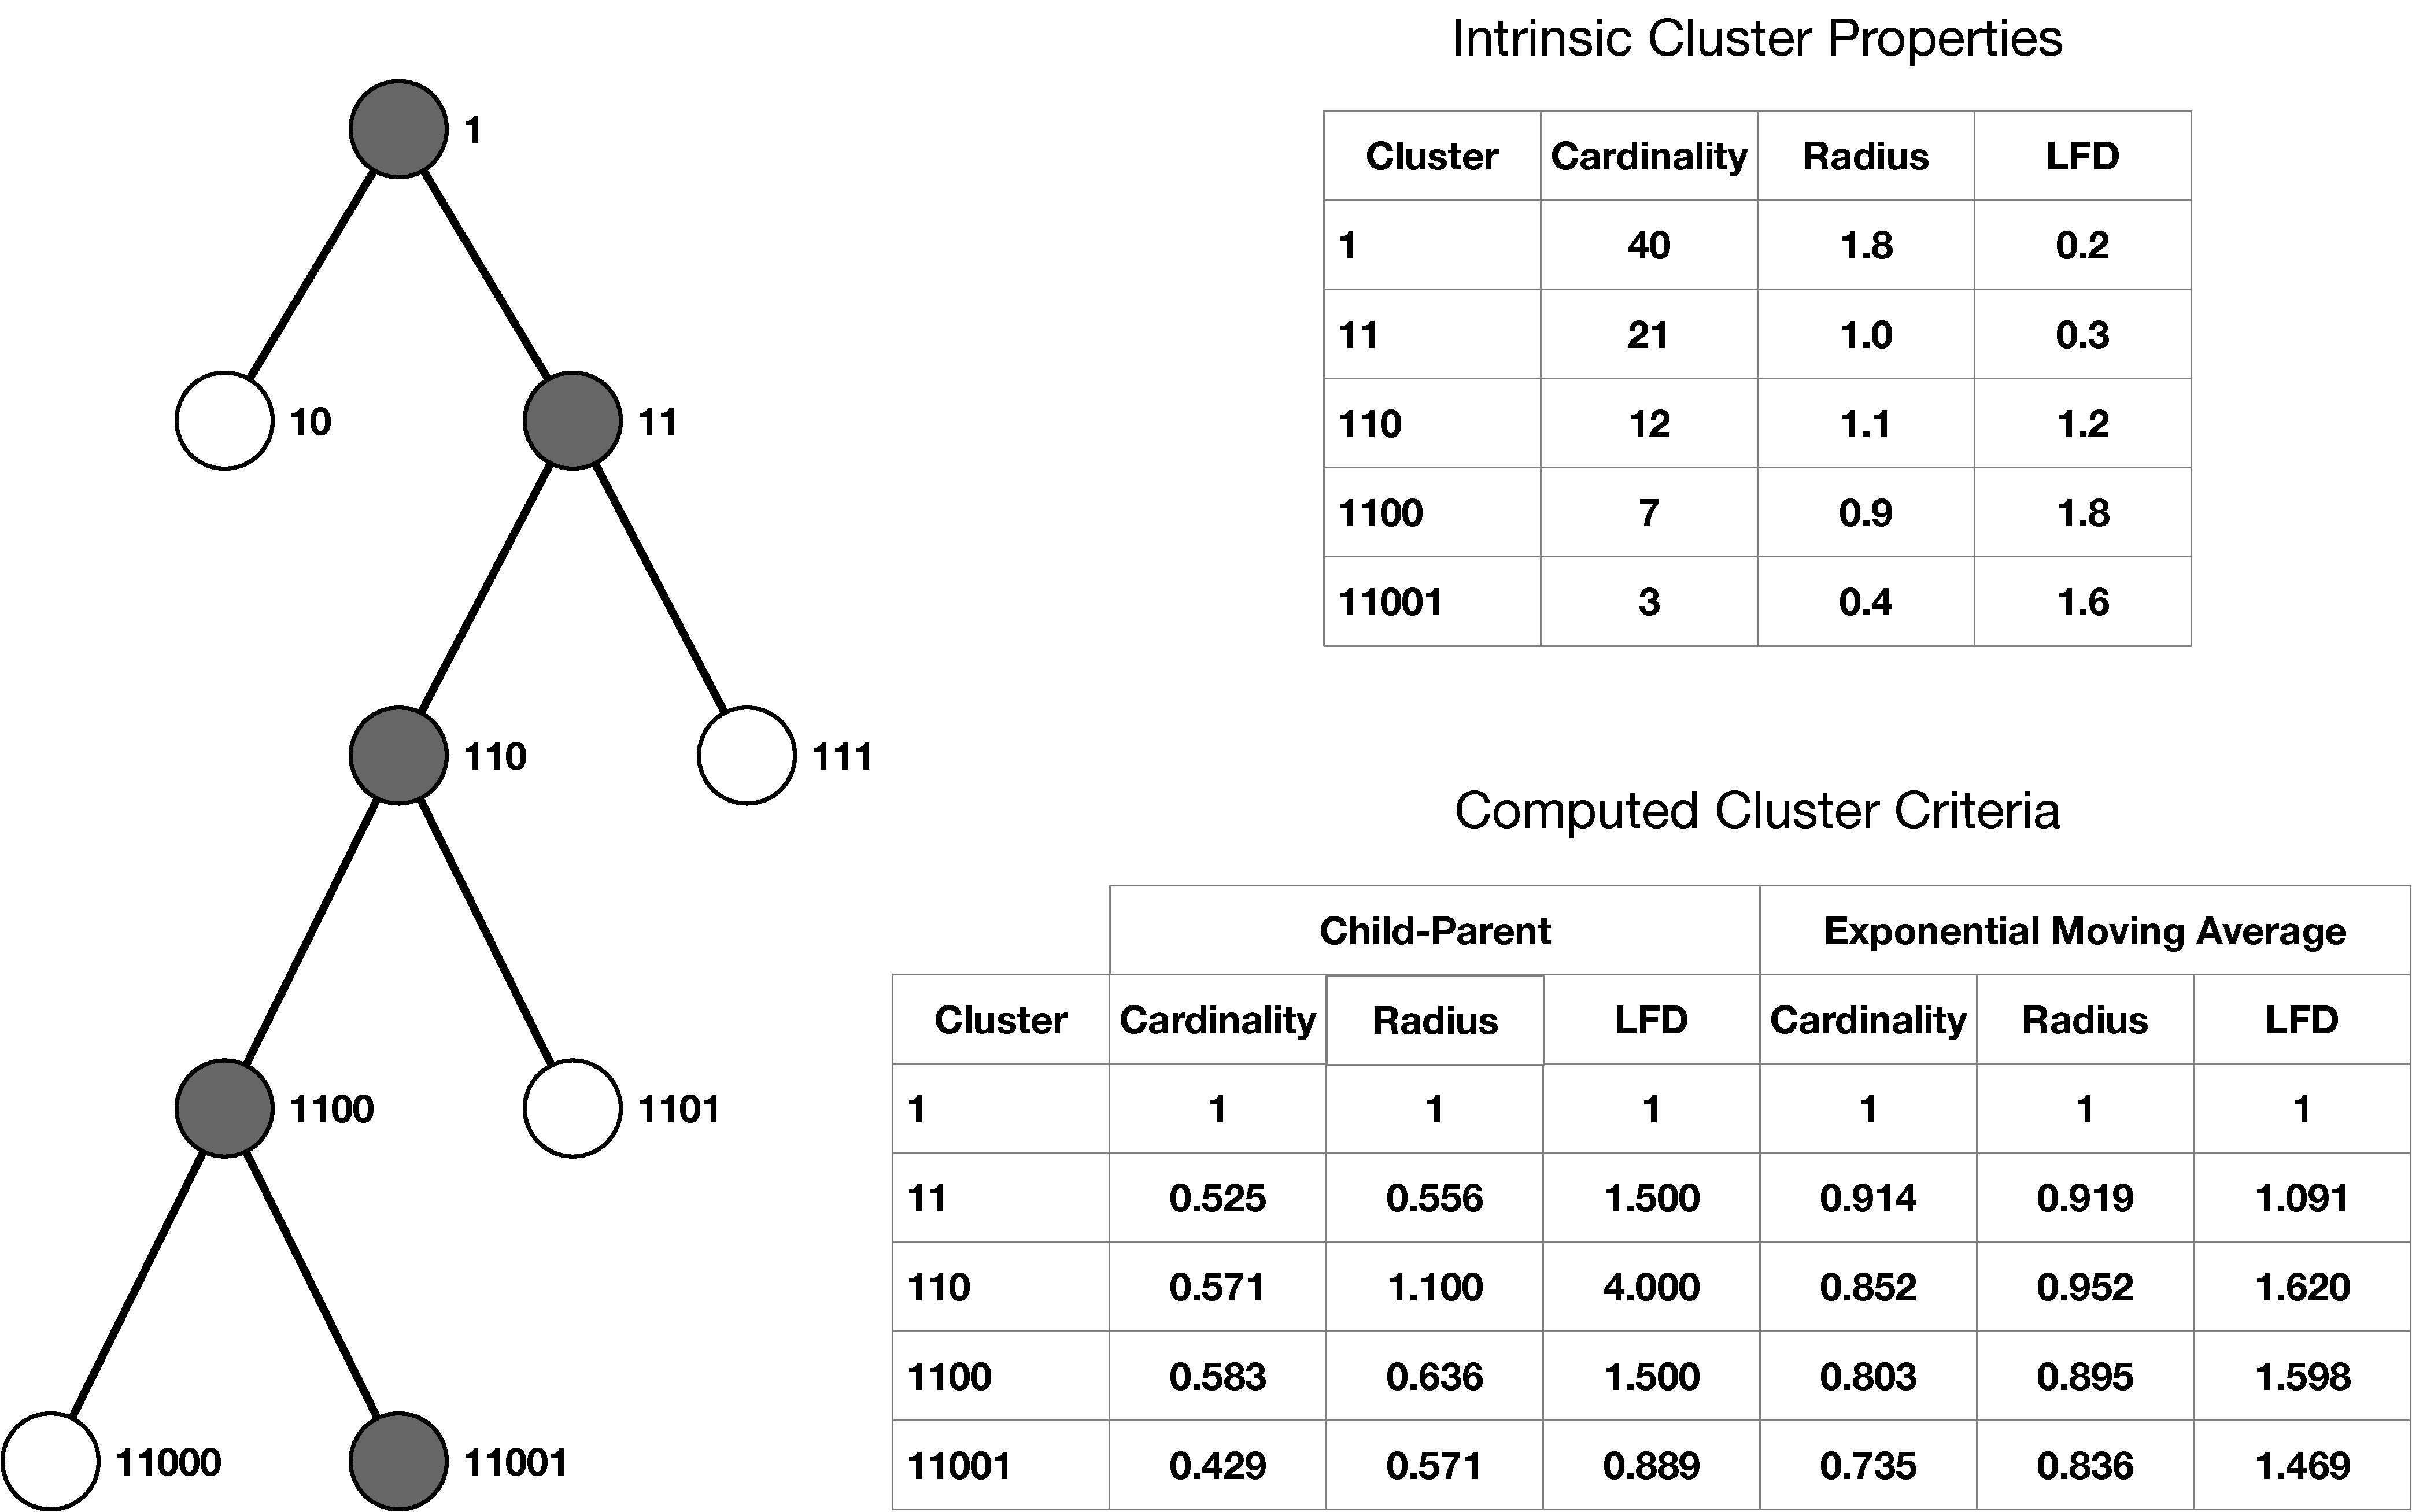
\includegraphics[width=2.5in]{images/chaoda-cluster-properties.pdf}
    \caption{
        \textbf{Cluster properties.}
        In the illustrated tree, we highlight only one branch for simplicity.
        We name the root `1' and we name the descendants as we might for a huffman tree.
        The upper table is an example of the values that intrinsic cluster properties might take on.
        The lower table shows the derived ratios we use for learning how to select clusters.
    }
    \label{fig:methods:cluster-properties}
\end{figure}

Specifically, we train a number of meta-ml models (see Section~\ref{subsec:methods:training-meta-ml-models} for details) and, from each model, we extract a function of the form $g : c \rightarrow \mathbb{R}$.
This function assigns high values to clusters which would increase ROC AUC and low values to clusters which would decrease ROC AUC.
As described in Algorithm~\ref{alg:cluster-selection}, the selection process begins by sorting, in non-increasing order, all clusters in the tree by the value assigned by $g$.
This sorting represents a ranking of the clusters for expected anomaly detection performance.
We iteratively select the best cluster from the rankings, and with each selection, we remove the ancestors and descendants of the selected cluster from the list of rankings.
Once the list of rankings is exhausted, we have selected the clusters with which to build an \textit{optimal graph}.

\begin{algorithm}[h]
    \caption{Cluster Selection}
    \label{alg:cluster-selection}
\begin{algorithmic}[1]
    \REQUIRE $T$, a cluster-tree
    \REQUIRE $g : c \rightarrow \mathbb{R}$ a ranking function
    \STATE $G \gets$ an empty graph
    \STATE $h \gets$ a list of all clusters $c \in T$ sorted by $g(c)$
    \REPEAT
        \STATE $c \gets$ pop\_first($h$)
        \STATE Add $c$ to $G$
        \STATE Remove all ancestors and descendants of $c$ from $h$
    \UNTIL $h$ is empty
\end{algorithmic}
\end{algorithm}



\subsection{The Ensemble}
\label{subsec:methods:the-ensemble}

During the testing and inference phases, we begin with a new dataset (not included in the training set of datasets) and one or more distance functions.
CLAM first builds cluster-trees using each distance function with the given dataset.
CHAODA uses the trained meta-ml models to select a different graph from each tree for each individual algorithm.
CHAODA applies each individual algorithm to its corresponding graph and produces anomalousness scores for each datum.
With two distance functions, six individual algorithms, and two meta-ml models, we can get up to $24$ different members with which to form an ensemble.
CHAODA normalizes the scores from all members and aggregates them, by their mean, into a final set of predictions for the anomalousness of each datum.


\subsection{Datasets and Comparisons}
\label{subsec:methods:datasets-and-comparisons}

We sourced 24 datasets containing only numerical features, i.e.\ not categorical features, from Outlier Detection Datasets (ODDS)~\cite{rayana2016odds}.
All of these datasets were adapted from the UCI Machine Learning Repository (UCIMLR)~\cite{UCIMLR}, and were standardized by ODDS for anomaly detection benchmarks.
Note that CHAODA is able to handle either entirely-numerical or entirely-categorical datasets, but not mixed datasets.
We discuss some future work relating to this in Section~\ref{sec:discussion}.

We randomly selected six datasets to train CHAODA: ann-thyroid, mnist, pendigits, satellite, shuttle, and thyroid.
The other eighteen datasets were used for testing and benchmarks: arrhythmia, breastw, cardio, cover, glass, http, ionosphere, lymphography, mammography, musk, optdigits, pima, satimage-2, smtp, vertebral, vowels, wbc, and wine.
We benchmarked CHAODA 30 times, using different random seeds, on the test set of datasets (see the Supplement at https://github.com/URI-ABD/chaoda for more details).
During testing, we noticed that even though we often see $|V| \ll n $, the graph neighborhood size and stationary probabilities methods from~\ref{subsec:methods:individual-algorithms} took prohibitively long to run, so we only use them when $|V| < max(128, \lfloor \sqrt n \rfloor)$.
We present these results in Table~\ref{table:results:test-performance} under the CHAODA-fast and CHAODA rows.
CHAODA-fast exhibits comparable performance to CHAODA, and we offer it as an option in our implementation.
All benchmarks were conducted on a 28-core Intel Xeon E5-2690 v4 2.60GHz, 512GB RAM and CentOS 7 Linux with kernel 3.10.0-1127.13.1.el7.x86\_64 \#1 SMP and Python 3.6.8.

We use the ground-truth labels only during the training phase with a small set of datasets.
Having once been trained, CHAODA becomes an unsupervised algorithm for any new dataset.
As such, we compared CHAODA only against other unsupervised algorithms.
We selected $18$ unsupervised algorithms from the pyOD suite~\cite{zhao2019pyod} and Scikit-Learn~\cite{pedregosa2011scikit}, as well as RS-Hash~\cite{sathe2016subspace}.
A supervised version of CHAODA is possible future work, which would open up comparisons against supervised or weakly-supervised methods such as REPEN~\cite{pang2018learning} and DAGMM~\cite{zong2018deep}.

For a ``Big-Data'' challenge, we ran CHAODA on the APOGEE2 data from the SDSS~\cite{blanton2017sdss}.
This dataset has a cardinality of $528,319$ and a dimensionality of $8,575$.
See Section~\ref{subsec:results:sdss-apogee2} for results.
All of these datasets were prepared by UCI and ODDS. 
In our experiments, we simply read them as 2-dimensional arrays where the columns are the features and the rows are the instances. 
We pre-processed the APOGEE2 data into a similar array, but of course it has no ground-truth labeling.
